%% ----------------------------------------------------------------
%% ProjectManagement.tex
%% ----------------------------------------------------------------
\chapter{Project Management}
\label{Chapter: Project Management}

\begin{preamble}
	Due to the large and complex nature of the project, care was taken to ensure the group's time and effort was managed effectively. This chapter gives details of how the group formed as well as the general positions within the team each member took. Information about the group's working procedure is given, along with details of how the group communicated internally and with project stakeholders.
	\preamblequote{Management is doing things right;\\leadership is doing the right things.}{Peter Drucker in \emph{Leadership}}
\end{preamble}

\section{Formation}
\label{Section:Formation}

Although as a whole the group had never worked together in the past, some existing close working relationships existed due to previous group coursework. As such it was easy to form the group and begin producing impressive results.

\subsection{Skills Audit}
\label{Section:Skills Audit}

Many of the strengths and weaknesses of the group members were clear from previous work, but a skills audit was undertaken to ensure that the group was competent to complete both the coursework and the project without fault.

To begin with, a requirement analysis was performed to determine exactly what skills were needed. These split into three clear subsections: management and leadership (from the perspective of both the coursework and the project); technical; and communication.

Next, an audit of each team member's skills was performed, the results of which can be found in \cref{App:Skills Audit Results}. From these an analysis of the group's total skills was determined, and the group's weaknesses could be found. It was found that the group had no clear weaknesses that could found using self-audit. Any members with a weakness were complemented by other members strengths.

\subsection{Roles and Responsibilities}

Throughout the project all members took on a number of project roles, both technical and management. Care was taken to allow for flexibility between and within roles. Roles and responsibilities were assigned dynamically, with members volunteering when they felt they were the best fit.

\begin{description}
	\item[Christopher Baines] \hfill \\
		Christopher focused on architectural design and component interaction. Much of his technical work was in-depth and complex in nature. His particular focuses were the Videogular Questions plugin and the analytics server.
	\item[Samuel Bennett] \hfill \\
		Samuel took a leadership role early in the project. He spent much of his time removing technical blockers for other members and acting as a central hub, keeping all members abreast with the work of others. Technically, he used his previous \gls{AngularJS} knowledge to begin work on the code bases for the project, as well as working closely with Christopher Baines in determining the general architectural design. Much of his technical work was done on Videogular Questions and the \gls{DF} format.
	\item[Harry Cutts] \hfill \\
		Harry's main technical contribution was the Videogular Cuepoints plugin, and the accessibility improvements that were contributed to \gls{Videogular}. He also ensured that the project work was being completed to a good standard, using coding conventions and tools such as JSHint. He also took on part of the role of Scrum Master, ensuring the group conformed to the agile process, and took minutes of group meetings.
	\item[Christopher Hewett] \hfill \\
		Christopher's technical work focused initially on the Videogular Questions plugin (in particular compatibility with mobile devices), and then later on the authoring tool. One of his earlier key themes was completing work on the styling of all front-ends. In the last few weeks prior to Christmas Christopher took on a leadership role in ensuring everything was completed on time.
	\item[Maria Lynch] \hfill \\
		Maria's technical contributions focused on the initial design and implementation of the authoring tool, and the design and implementation of the Videogular Heatmap plugin. Maria took responsibility for organising the coursework deliverables. She managed the report production, and also contributed to the user interface design and accessibility of many of the deliverables.
\end{description}

Generally the group felt that all members completed similar amounts of work over the course of the project, as well as sharing equal responsibility.

\section{Project Process}
\label{Section:Project Process}

The project was run using an agile methodology based on Scrum. This involved having weekly sprints where each person completed a number of tasks, either alone or collaborating with others. Planning meetings were held at the start of each sprint where the issues in the backlog were discussed, prioritised, and given a point value related to how much time it would take to resolve. The issues were then assigned to one or more group members, in order of priority. Each person had a maximum capacity of points for each week. At the end of each sprint, a retrospective was held to discuss the previous sprint and the way in which the project management was being carried out.

This structure meant that the planning and monitoring of the project happened formally on a sprint by sprint basis. When required the group adapted their working practices, without being constrained by the Scrum model. For example, when preparing for progress presentations ``mini-sprints'' were run both for the presentation and for work to be completed in the remainder of the week.

Figure \cref{ganttChart1} and \cref{ganttChart2} show the project progress.
They slightly deviate from the original plan (\autoref{App:Gantt Charts})

\begin{landscape}

\ganttset{%
    calendar week text={%
        W~\currentweek%
    }%
}

\begin{figure}[h!]
\begin{ganttchart}[
    hgrid,
    vgrid,
    x unit=1.8mm,
    time slot format=isodate
    ]{2014-09-29}{2014-12-14}
    \gantttitlecalendar{year, month, week=1} \\

    \ganttbar{Prototyping}{2014-09-29}{2014-10-12} \\
    \ganttgroup{Weekly Sprints}{2014-10-13}{2014-12-14} \\
    \ganttbar{Quiz and poll display component}{2014-10-13}{2014-11-16}\\
    \ganttmilestone{Progress Seminar 1}{2014-10-22} \\
    \ganttbar{Authoring tool}{2014-10-20}{2014-12-14}\\
    \ganttbar{Analytics tool}{2014-11-10}{2014-12-14}\\
    \ganttmilestone{Progress Seminar 2}{2014-11-19}\\
    \ganttmilestone{Agree deliverables with customer}{2014-12-14}
\end{ganttchart}

\caption{Gantt Chart prior to the Christmas vacation.}
\label{ganttChart1}
\end{figure}

\begin{figure}[h!]
\begin{ganttchart}[
    hgrid,
    vgrid,
    x unit=1.8mm,
    time slot format=isodate
    ]{2014-12-15}{2015-02-22}
    \gantttitlecalendar{year, month, week=12} \\

    \ganttgroup{Christmas}{2014-12-15}{2015-01-04} \\
    \ganttgroup{Exams}{2015-01-12}{2015-01-24} \\
    \ganttbar{Group report finalisation and review}{2015-01-05}{2015-01-29}\\
    \ganttmilestone{Group Report}{2015-01-29} \\
    \ganttbar{Individual reflection}{2015-01-25}{2015-02-02}\\
    \ganttmilestone{Individual Reflection submission}{2015-02-02} \\
    \ganttbar{Poster and Presentation creation}{2015-01-30}{2015-02-05}\\
    \ganttmilestone{Poster and Presentation submission}{2015-02-05} \\
    \ganttbar{Presentation rehearsal}{2015-02-03}{2015-02-11}\\
    \ganttmilestone{Final Presentation}{2015-02-11}
\end{ganttchart}

\caption{Gantt Chart after the  Christmas vacation}
\label{ganttChart2}
\end{figure}

\end{landscape}

Due to the use of version control and issue tracking, it is easy to produce retrospective statistical analysis.

By tracking commits within the GitHub organisation (over 1000) one can determine when the week's work was normally completed. This data is visualised in \autoref{fig:punch card}. It is important to remember that work occurs prior to a commit and as such the commit time is an ending marker. Looking at \autoref{fig:punch card} one can see the group generally completed most of their work as it would have been done in an industrial setting, during standard office hours, with extra work being done late into the evenings and on weekends.

%http://tex.stackexchange.com/questions/86114/github-like-punchcard-with-the-help-of-pgfplots
\begin{figure}
  \makebox[\textwidth][c]{
\begin{tikzpicture}                                             %1
        \begin{axis}[                                               %2
                grid=major,                                         %3
                point meta=explicit,
                xmin=-1,
                xmax=24,
                xlabel=Hours,                                       %7
                scatter/@pre marker code/.code={
                    \pgfmathparse{                                  %12
                        sqrt(\pgfplotspointmetatransformed)/50*12}   %13
                    \def\markopts{                                  %14
                        mark=*,                                     %15
                        color=black,                     %16
                        fill=black,                      %17
                        mark size=\pgfmathresult}                   %18
                    \expandafter\scope\expandafter[\markopts]},
                scatter/@post marker code/.code={
                    \endscope},
                symbolic y coords={Sun,Sat,Fri,Thu,Wed,Tue,Mon},
                xtick={0,...,23},
                x=0.55cm,
                y=0.9cm]
            \addplot[only marks,scatter]
                table[x index=0, y index=1, meta index=2] {punchcard.dat};
        \end{axis}
\end{tikzpicture}
  }%
  \caption{A punch card diagram showing the frequency of commits at different hours of the day. The area of each circle is proportional to the number of commits.}
  \label{fig:punch card}
\end{figure}

By tracking closed issues on a week by week basis it is possible to determine when work was completed throughout the project. Although issues are of different sizes, over the sample of 100s of issues a general grasp can be achieved. A graph of this can be seen in \autoref{fig:tasksweek}. It shows that work was completed steadily throughout the semester. Week 8's deficiency can be explained by the issues being more time consuming, as well as the second progress presentation and other coursework needing to be completed that week. The dip between weeks 12 to 17 is explained by the Christmas break and examination period.

%Sam has the code to generate this from the GitHub API
\begin{figure}
\centering
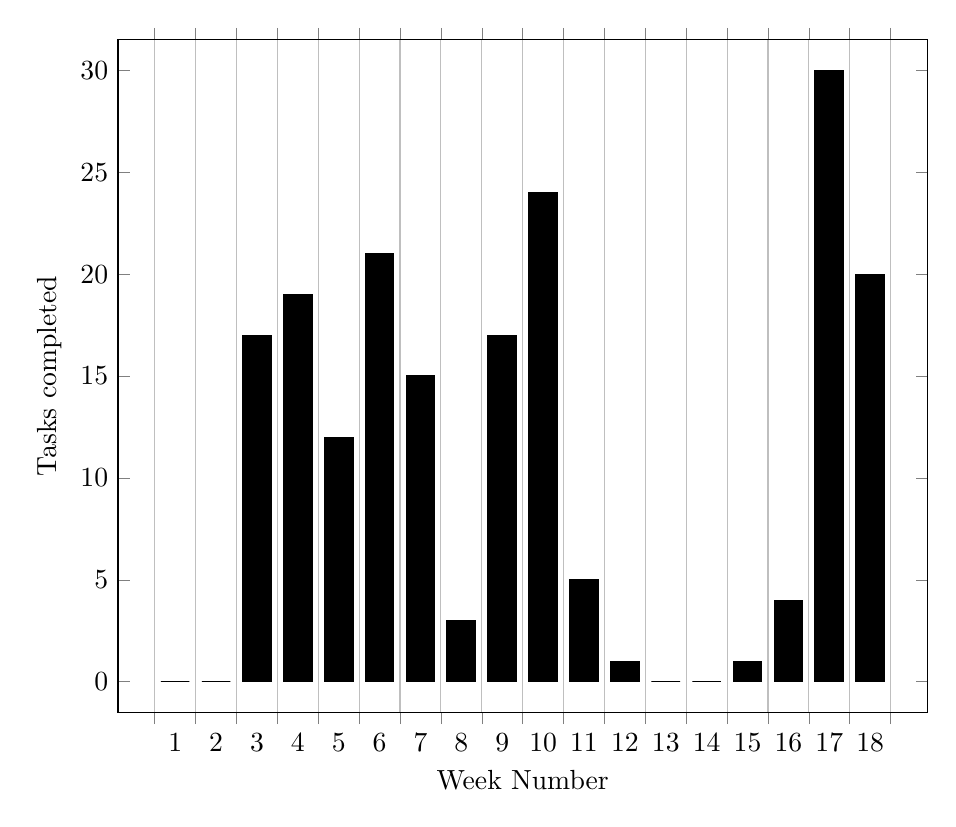
\begin{tikzpicture}
\begin{axis}[
	scale=1.5,
	ylabel={Tasks completed},
	xlabel= {Week Number},
	enlargelimits=0.05,
	ybar interval=0.7,
]
\addplot[black,fill=black]
	coordinates {(1, 0) (2, 0) (3, 17) (4, 19) (5, 12) (6, 21) (7, 15) (8, 3) (9, 17) (10, 24) (11, 5) (12, 1) (13, 0) (14, 0) (15, 1) (16, 4) (17, 30) (18, 20) (19,0)};
\end{axis}
\end{tikzpicture}
  \caption{A bar chart of the number of GitHub issues being closed in each week of the project.}
  \label{fig:tasksweek}
\end{figure}


\subsection{Collaboration and Issue Management}
To allow for collaborative work a GitHub organisation\footnote{\url{https://github.com/soton-ecs-2014-gdp-12/}} was used. This acted as a central repository not only for code and conventions documents, but also for presentations and reports. Separate repositories for each area of the project are located here for ease of access. Using GitHub made it easier to interact with other open source projects, and all pull requests and releases were directed from here.

GitHub also provided an issue management system on a repository by repository basis. This allowed tracking of conversations around different bugs and enhancements as the project progressed. The group used the Waffle.io\footnote{\url{https://waffle.io}} dashboard to manage the issues backlog from a project wide perspective as this would interface directly with GitHub.


\section{Client Management}
\label{Section:Client Management}

The project had a reasonably large number of stakeholders who needed to be managed and kept informed. Each stakeholder required different levels of communication via different methods.

The most important stakeholder was the client, Professor Mike Wald. Weekly meetings were organised, minutes of which can be found in \cref{App:Minutes of Meetings}, and emails were used for urgent issues.

Final project sign-off to check for client satisfaction was gathered using a deliverable report. It was delivered prior to the sign-off meeting and then discussed. It can be found in \cref{App:Deliverable Report}.

Another important stakeholder was Yunjia Li. He attend the weekly meetings as much as possible so as to ensure his future interests in the framework were protected. He was also contactable via email when necessary.

2fdevs, the Videogular development team, were communicated with via Gitter\footnote{\url{https://gitter.im/2fdevs/videogular}}, an online chat system integrated with GitHub. They had an ongoing interest with the framework due to its role of advertising the \gls{Videogular} project. Their advice and code proved invaluable throughout the project.

Shameem Bajar provided valuable user feedback. She came to meetings and communicated with the group via email.

\section{Management Problems}

Throughout the project a number of management problems were encountered and worked around.

Two weeks before the Christmas break, in week 10, Samuel Bennett suffered a bereavement in the family. As such he was unavailable for the whole of week 10. Upon learning this the group quickly restructured its leadership with Christopher Hewett taking responsibility. The team planned for Samuel to not return before Christmas, although this was not the case.

In the first few sprints the group found that the point value each member was supposed to complete had to be adjusted. Initially it was too low, meaning that all members did not have enough work assigned to them. This meant that people had to be flexible and use their own judgement in prioritising additional tasks for them to complete. In later weeks the point value allocation was increased.

At times the agile methodology was rather restricting. In particular issues were found around the presentation and report deliverables. To combat this the group adapted to ``mini-sprints''. This was needed as the presentation dates were halfway through the sprint window (Monday to Sunday). During these ``mini-sprints'' the week was broken up, with the first ``mini-sprint'' working towards the presentation and the second doing smaller pieces of work and documentation tasks.

One difficult problem was the inability to plan around other coursework for other modules. Within the group there were 14 additional pieces of coursework with ranging deadlines. Sometimes these deadlines were rather short or the amount of work required unclear. This made the weekly planning process difficult at times, requiring the group to be sympathetic to its members and accommodate change as needed. However, the agile project planning methods meant flexibility and success could be achieved.
